\documentclass[9pt,twocolumn,twoside]{../../styles/osajnl}
\usepackage{fancyvrb}
\usepackage{hyperref}
\usepackage{booktabs,caption}
\usepackage[flushleft]{threeparttable}
\usepackage{color}
\usepackage{listings}
\lstdefinestyle{BashInputStyle}{
  language=bash,
  basicstyle=\small\sffamily,
  numbers=left,
  numberstyle=\tiny,
  numbersep=3pt,
  frame=tb,
  columns=fullflexible,
  backgroundcolor=\color{yellow!20},
  linewidth=0.9\linewidth,
  xleftmargin=0.1\linewidth
}
\journal{i524} 

\title{Remotely Deploying, Visualizing and Controlling a Robot Swarm with ROS and Cloudmesh}

\author[1]{Matthew Lawson}
\author[1,*]{Gregor von Laszewski}

\affil[1]{School of Informatics and Computing, Bloomington, IN 47408, U.S.A.}

\affil[*]{Corresponding authors: laszewski@gmail.com}

\dates{Project: S17-IO-3010, \today}

\ociscodes{Cloud, I524, ROS, Gazebo, Robot, Swarm}

% replace this with your url in github/gitlab
\doi{Report: \url{https://github.com/cloudmesh/sp17-i524/tree/master/project/S17-IO-3010/report/report.pdf}\\
Code: \url{https://github.com/cloudmesh/cloudmesh.ros}}

\begin{abstract}
Working with robot swarms is one important research area of robotics. To educate the next generation experts we are in the need to simulate large such swarms as the cost to deploy them as real hardware may be prohibitive to a university with limited budget. Hence, we explore the the feasibility of simulating such swarms while harnessing remotely-located distributed computing environments to conduct such simulations. We are especially interested to reuse clouds to simulate large-scale robot swarms.  For this reason we created a proof-of-concept that creates a two-robot swarm on multiple clouds we have access to.  The important point is the the deployment is done automated and can be executed by non cloud experts so the environment is accessible and usable not only by advanced PhD students, but by freshmen and potentially even STEM students. The robots behaviour are streemed as a visual simulation the remote user.  We demonstrate that users can start up the behavior of a robot through a single command allowing us to benchmark the activity streams of the swarm in tehe cloud. The project uses opensource software and utilizes Open Source Robotics Foundation (OSRF) to define, create and control the virtual robots with \textit{Robot Operating System}.  \textit{Gazebo} provides the visualization of the simulation.  To simplify the interaction with various clouds we use \textit{cloudmesh}.
\end{abstract}

\setboolean{displaycopyright}{false}

\begin{document}

\maketitle

\section{Introduction}
With the evolution of robotics and its increased influence in society we anticipate the need to deal with robot swarms. Thus, we need to educate the next generation of scientists by offering abilities to simulate a multitude and diverse set of robot swarms. Simulation allows safe interaction with the swarm while conducting actions and observing responses to its environment prior to real-world deployment to mitigates operational risk. Furthermore it allows to simulate such environments in a cost effective way that goes beyond the capabilities that are provided by a single workstation. The question we ask, would it be possible to simulate 10th of thausends of robots on a cloud environment?

However, deployment of an interconnected swarm of virtual robots in a cloud imposes additional requirements to the scientist researching such swarms. Thus we try to also evaluate if it is possible to bring down the barrier of managing such a {\em virtual swarm} not only for an individual researcher but for potential inclusion in class settings on the freshmen and the STEM level. Although cloud environments are available today accessing and configuring multiple computers presents a time and resource challenge in contrast to a single-host setup.  In addition, network security measures, such as ssh keys and port access, impede ROS' intra-cluster communication capabilities.  These aspects are typically out of reach for such entry level educational communities. In order to address the unique requirements of a networked, remotely-located swarm, we create a multi-platform system to automate the creation and deployment of the virtual swarm with the help of cloudmesh \cite{??}.

\section{Virtual Robot Swarm Components}

\subsection{Robot Operating System (ROS) \cite{paper2}}

\begin{figure*}[htbp]
\centering
\fbox{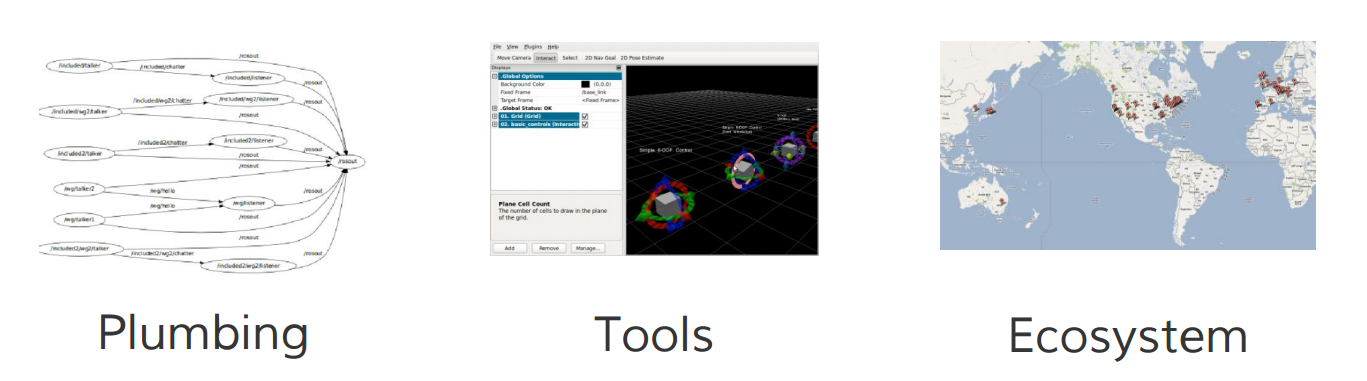
\includegraphics[width=\linewidth]{images/ros-is.png}}
\caption{A Conceptualization of What ROS, the \textit{R}obot \textit{O}perating \textit{S}ystem, Offers to Roboticists \cite{www-ros-ros-is}}
\label{fig:rosOverview}
\end{figure*}

\begin{figure}[htbp]
\centering
\fbox{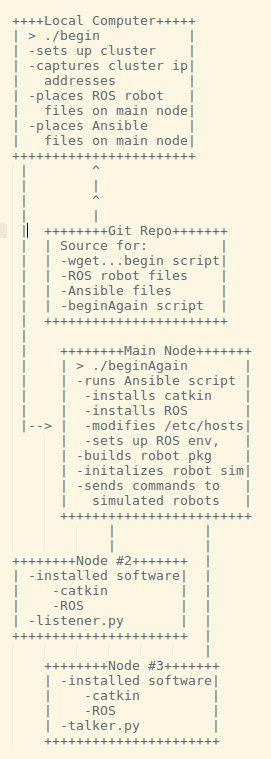
\includegraphics[width=\linewidth]{images/deployWorkFlowCol.jpeg}}
\caption{Deployment Workflow for the Virtual Robot Swarm Project}
\label{fig:deployWorkflow}
\end{figure}

The Open Source Robotics Foundation's middleware product \textit{Robot Operating System}, or ROS, provides a framework for writing operating systems for robots.  ROS offers ``a collection of tools, libraries, and conventions [meant to] simplify the task of creating complex and robust robot behavior across a wide variety of robotic platforms'' \cite{www-ros-about}. The Open Source Robotics Foundation, hereinafter OSRF or the Foundation, attempts to meet the aforementioned objective by implementing ROS as a modular system.  That is, ROS offers a core set of features, such as inter-process communication, that work with or without pre-existing, self-contained components for other tasks.

Figure 1 depicts the three parts of the ROS universe: a) the plumbing, ROS' communications infrastructure; b) the tools, such as ROS' visualization capabilities or its hardware drivers; and c) ROS' ecosystem, which represents ROS' core developers and maintainers, its contributors and its user base.

The modules or packages, which are analogous to packages in Linux repositories or libraries in other software distributions such as \textit{R}, provide solutions for numerous robot-related tasks and challenges.  General categories include a) drivers, such as sensor and actuator interfaces; b) platforms, for steering and image processing, etc.; c) algorithms, for task planning and obstacle avoidance; and, d) user interfaces, such as tele-operation and sensor data display. \cite{www-software-categories}

\subsubsection{Communications Infrastructure}
\paragraph{General}
OSRF maintains three distinct communication methods for ROS: a) \textit{message passing}; b) \textit{services}; and, c) \textit{actions}.  Each method utilizes ROS' standard communication type, the \textit{message} \cite{www-ros-core-components}.  Messages, in turn, adhere to ROS' \textit{interface description language}, or IDL. The IDL dictates that messages should be in the form of a data structure comprised of typed fields \cite{www-ros-messages}. Finally, \textit{.msg} files store the structure of messages published by various nodes so that ROS' internal systems can generate source code automatically.  The virtual swarm and the talker/listener robots utilize ROS' message passing capabilities in project's this implementation.

\paragraph{Message Passing}
ROS implements a publish-subscribe anonymous message passing system for inter-process communication, hereinafter pubsub, as its most-basic solution for roboticists.  A pubsub system consists of two complementary pieces: a) a device, node or process, hereinafter node, publishing messages, i.e., information, to a \textit{topic}; and b) another node \textit{listening to} and ingesting the information from the associated topic.  Designating topics to which a node should subscribe and topics to which a node should publish falls to the roboticist.  ROS' \textit{rosnode} command line tool conveniently "display[s] a list of active topics, the publishers and subscribers of a specific topic, the publishing rate of a topic, the bandwidth of a topic, and messages published to a topic" \cite{www-ros-rostopic}.

Pubsub's method of operation analogizes to terrestrial radio.  In the analogy, the radio station represents the publishing node, the radio receiver maps to the subscribing node and the frequency on which one transmits and the other receives represents the topic.  Unlike terrestrial radio, though, ROS provides a lookup mechanism versus "flipping through the dial."

The OSRF touts the pubsub communications paradigm as the ideal method  primarily due to its anonymity and its requirement to communicate using its message format.  With respect to the first point, the nodes involved in bilateral or multilateral conversations need only know the topic on which to publish or subscribe in order to communicate.  As a result, nodes can be replaced, substituted or upgraded without changing a single line of code or reconfiguring the software in any manner.  The subscriber node can even be deleted entirely without affecting any aspect of the robot except those nodes that depend on the deleted node.

In addition, ROS' pubsub requires well-defined interfaces between nodes in order to succeed.  For instance, if a node publishes a message without a crucial piece information a subscribing node requires or in an unexpected format, the message would be useless.  Alternatively, it would be pointless for an audio processing node to subscribe to a node publishing lidar data.  Therefore, a message's structure must be well-defined and available for reference as needed in order to ensure compatibility between publisher and subscriber nodes.  As a result, ROS has a modular communication system.  That is, a subscriber node may use all or only parts of a publishing node's message.  Further, the subscribing node can combine the data with information from another node before publishing the combined information to a different topic altogether for a third node's use.  At the same time, a fourth and fifth node could subscribe to the original topic for each node's respective purpose.  

Finally, ROS' pubsub can natively replay messages by saving them as files.  Since a subscriber node processes messages received irrespective of the message's source, publishing a saved message from a subscriber node at a later time works just as well as an actual topic feed.  One use of asynchronous messaging: postmortem analysis and debugging.

\subsection{Gazebo} 
The Foundation also supports \textit{Gazebo}, ROS' 3D virtual simulation software.  ``Gazebo...simulate[s] populations of robots in complex indoor and outdoor environments. [It] offers physics simulation at a much higher degree of fidelity [than gaming engines], a suite of sensors, and interfaces for both users and programs \cite{www-gazebo-overview}.''  Gazebo's usefulness center on three main features: a) physics engines compatibility; b) its graphics engine; and c) its sensor-data generators.  with respect to physics engine compatibility Gazebo interfaces well with \textit{Open Dynamics Engine} \cite{www-ode-homepage} (ODE), the default; b) \textit{Bullet} \cite{www-bullet-homepage}; \textit{SimBody} \cite{www-simbody-homepage}; and, \textit{DART} \cite{www-dart-homepage}. Roboticists also benefit from its 3D graphics engine, \textit{Object-oriented Graphics Rendering Engine} \cite{www-ogre-homepage} (OGRE), which provides a C++ class library to ``[abstract away] the details of using the underlying [graphics] system libraries like Direct3D and OpenGL \cite{www-ogre-about}.''  Finally, Gazebo can supply \textit{sensor} data to the virtual robot.  Virtual sensor support ranges from 2D cameras to Kinect-style sensors.  The system can also generate \textit{noisy} data to better simulate real-world results.

Gazebo exists as a stand-alone project, suitable for use by programs other than ROS.  However, it integrates tightly with ROS given its common ownership.  In fact, the version supplied with a ROS installation automatically establishes communications between Gazebo and ROS for the end-user \cite{www-gazebo-ros}.

\subsection{Ansible}
Red Hat, Inc's \cite{www-redhat} \textit{Ansible} software purports to simplify numerous information technology tasks.  It claims to do so by a) relying upon a human-readable script syntax, YAML; and b) by automating definable and repeatable IT tasks, such as configuration management and application deployment.  Ansible's developers adopted a theater metaphor to describe the program's core functions.  Thus, a computer's main duty within an IT infrastructure corresponds to the \textit{role} an actor or actress might play in a theatrical production.  Ansible calls the script a \textit{playbook}, while the lines and directions within the script are referred to as \textit{tasks}.  Other aspects diverge from the metaphor, such as group vars and the config file (ansible.cfg).  However, the \textit{inventory} file hews to the metaphor - it represents the cast billing, the delineation of who plays what role.  When used with an Ansible playbook, the inventory file specifies which servers belong to which logical group(s), i.e., which role(s). 

As a result the software's applicability extends well beyond simplistic tasks even though Ansible's designers strive for simplification.  In fact, an Ansible user can exercise fine-grained control over nearly every aspect of his or her IT infrastructure with a well-designed playbook.  

Ansible also attempts to ease the burden of the IT administrator by eschewing SSL signing servers, daemons or client software.  It simply pushes small programs to the target computers through an SSH connection to execute the desired tasks.  When the task completes, Ansible removes the programs. 

\subsection{cloudmesh client toolkit}
The \textit{cloudmesh client toolkit} (cm) attempts to abstract away the complexities of establishing and utilizing different remotely-accessed computers and computer clusters \cite{www-cm}.  Users can create, access and destroy a virtual machine or cluster of machines by issuing a single line of commands from a terminal emulator.  cm supports access to clouds based on various back end-software stacks, including SLURM, SSH, Openstack and Heat.  It provides an API, a command line client and a shell client.

\subsection{Testing Environment}
The Chameleon project's cluster of 650+ multi-core computer nodes, a joint venture between the University of Chicago and the Texas Advanced Computing Center, provides the infrastructre for the project.  It is colloquially referred to as Chameleon Cloud or CC.  A 100Gbps connection runs between the two centers. Project development primarily occurred on three-node clusters created as needed using Chameleon Cloud's \textit{m1.medium} flavor of Ubuntu 16.04.  Deployment testing also utilized the \textit{m1.xlarge} and \textit{m1.xxlarge} flavors CC provides.

% \begin{table} [htbp]
%   \begin{threeparttable}
%   \centering
%   \caption{Deployment Resources}
%     \begin{tabular}{cccc}
%       \multicolumn{4}{c}{\bf Chameleon Cloud Flavor Specifications}\\ \hline Flavor & vCPU & RAM & Hard Drive \\ \hline m1.medium & 2 & 4 & 40\\ m1.large & 4 & 8 & 80 \\ m1.xlarge & 8 & 16 & 160 \\ \hline
%     \end{tabular}
%     \begin{tablenotes}
%       \small
%       \item \textit{vCPU}: count of virtual CPUs; RAM units: MB; Hard Drive units: GB 
%     \end{tablenotes}
%   \end{threeparttable}
% \end{table}

\subsection{Robots and Worlds with ROS}
A ROS robot may be extremely simple, such as the pre-built talker and listener robots supplied in the ROS distribution, or as complex as the roboticist desires.  If users desire to visualize the robot, s/he must define his / her ROS robot in \textit{\textbf{U}niversal \textbf{R}obot \textbf{D}escription \textbf{F}ormat}.  A ROS robot's specifications reside in a series of files with \textit{xacro} extensions, referred to as URDF files.  These files, which borrow XML's syntax structure, can include specifications for the basic shapes of the robot and its appendages (if applicable), e.g., rectangular box, cylinder, etc. with attached wheels; various kinds of joints, such as ones that rotate around an axis or extend along an axis; types and numbers of sensors; number of joints in an appendage; colors of the robot(s); etc., etc.  In addition, any file in the robot description stack may reference an external file to complete the description of the robot.  This capability allows the user to re-use code by incorporating previously-completed robot features into a new robot.  Finally, simulations include a world file to provide the setting, or environment, in which the robot simulation occurs.  As with the URDF files, the world file can be simple, like the \textit{empty\_world} file included in the ROS distribution or extremely complex.  

Finally, a simulation package will include one or more \textit{launch} files.  These files coordinate the disparate aspects of the entire simulation package in a manner similar to that of Ansible's playbook file.  According to the OSRF, best practices for robot simulation dictate that the main launch file consist of little more than calls to other launch files in the package \cite{www-ros-launch}.  Continuing with the playbook analogy, the launch files called from the main launch file would correspond to the roles defined in Ansible.  This functionality significantly increases ROS' usability since managing even relatively straightforward robots, simulated or real, can prove unwieldy. For instance, this project, a proof-of-concept project, utilizes a .world file, four URDF files and four launch files in addition to the pre-compiled talker and listener robots.  

This project uses two straightforward differential drive robots sourced from an online tutorial entitled \textit{Simulating Robot Models in ROS (part 1)} \cite{www-mybot-moore}

\section{Virtual Robot Swarm Project Implementation}
\subsection{VR Swarm task}
Although the swarm accomplishes the seemingly-trivial task of driving in circles, the real accomplishment rests in proving the feasibility of automating the deployment of multiple controllable virtual robots on a remote cluster of computers and then visualizing them on a local computer.

\subsection{Deployment}
Achieving the aforementioned task requires coordinating a modestly-complex mix of shell commands, cloudmesh commands, Ansible commands and ROS / Gazebo commands. A shell script provides the automation for the shell, cloudmesh and ROS commands, while Ansible's \textit{playbook} functionality handles the Ansible-focused portion.  Only the initial step, retrieving and sourcing the shell script that begins the deployment process, requires user intervention.  However, if the user wants to listen to the talker robot (\textit{talker.py and listener.py}), s/he needs to follow the steps described in the README file.

\begin{figure}[htbp]
\centering
\fbox{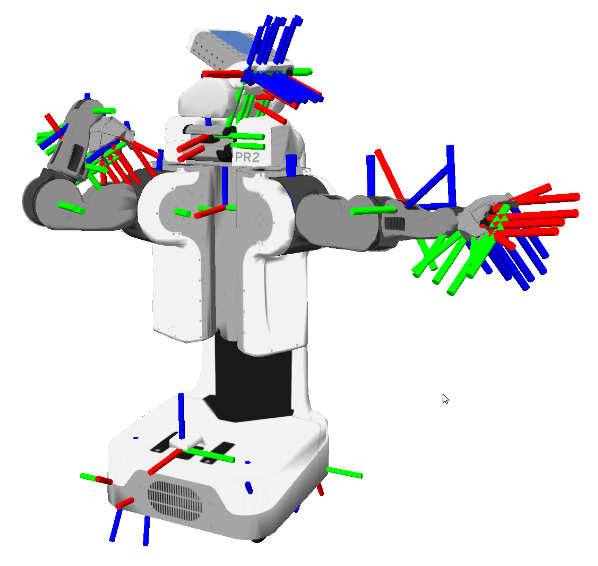
\includegraphics[width=\linewidth]{images/robotgeometry.png}}
\caption{Example of a Complex Simulated Robot}
\label{fig:complexRobot}
\end{figure}

\begin{figure}[htbp]
\centering
\fbox{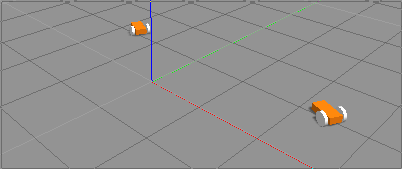
\includegraphics[width=\linewidth]{images/rosProjRobots.png}}
\caption{An Example of Two Simpler Robots}
\label{fig:simplerRobots}
\end{figure}

\paragraph{\textit{wget...begin} - Retrieve the Initalization Bash Script}
Deployment begins when the user retrieves the initalization file, named \textit{begin}, from the project's Github repository.  The user then starts the execution sequence by sourcing the file with the command

{\color{black} \lstinline[style=BashInputStyle]!> ./begin! }

from the directory where the \textit{begin} bash script resides.  

\paragraph{\textit{begin} bash script}
The bash script calls three cloudmesh\_client commands: 

\begin{enumerate}
\setlength\itemsep{-6pt}
\item {\lstinline[style=BashInputStyle]!> cm cluster define -n rosA1 -c 3! }
\item {\lstinline[style=BashInputStyle]!> cm cluster allocate! } 
\item {\lstinline[style=BashInputStyle]!> cm cluster cross_ssh! } 
\end{enumerate}

The script creates and prepares a three-node cluster named \textit{rosA1}.  
We then use two additional Cloudmesh commands:

\begin{enumerate}
\setlength\itemsep{-6pt}
\item  {\lstinline[style=BashInputStyle]!> cm cluster nodes! } 
\item  {\lstinline[style=BashInputStyle]!> cm vm ip show! } 
\end{enumerate}

to capture the public and private ip addresses of the cluster, as well as the host names.  

The ip addresses and names are written to separate files for distinct purposes.  The host names and private ip addresses are used to create a file to append to each cluster node's \textit{known\_hosts} file.  The private ip addresses also end up in a different file that serves as the basis for a custom Ansible inventory file.  

The private ip addresses, termed static ips by Chameleon, must be used because ROS nodes communicate by binding to any available port.  That is, ROS does not specify the port beforehand, and it does not consider whether or not the firewall blocks the port for security purposes.  As a result, intra-cluster communication requires access to every port, i.e., the firewall cannot close any port on any computer running ROS when that computer needs to communicate with another computer in the cluster.  Obviously, this presents a major security concern, especially on shared resources. Refer to the \textit{Deployment Obstacles} section below for the workaround used with this project.

As its penultimate step, the \textit{begin} script places all the necessary files for the demonstration on the correct cluster nodes.  The ROS robot files and the Ansible files go onto the main node, while the script places a copy of the known\_hosts addendum onto each cluster node.  In addition, the script uses the \textit{wget} command to copy the bash script for the next step in the process onto the main node.

The final lines of the file initiate the next step in the process, running the \textit{beginAgain} script on the master node, and perform a few administrative duties.

\paragraph{\textit{beginAgain} bash script}
This script handles the software installation and initialization of the robots.  It first establishes the veracity of the main node and the other nodes by connecting to each one in turn via ssh connection.  If these steps do not occur before Ansible runs, the software installations never occur because Ansible hangs mid-process.  Ansible installs all the necessary software on each cluster node.  It installs Linux's \textit{tree} package because the author prefers to use it to view directory structures; the ROS package; the rosbash package; the rosinstall package; and, the catkin\_tools package. Ansible also creates a new known\_hosts file for each computer node.

Upon completing the installation, the file's instructions initialize the robot workspace.  The \textit{catkin\_tools} package accomplishes this on behalf of ROS.  catkin\_tools represents an evolution of ROS' built-in \textit{catkin} family of commands.  Initializing the robot workspace essentially involves the addition of numerous hidden helper files, which assist in building the robot package.  Creating the robot package, referred to as \textit{building} the package, involves a series of automated \textit{CMake} commands.  

With the robot package built, the script copies another script from github.  This small script starts ROS' \textit{talker} robot, a simple robot included as part of ROS' tutorial packages.  It relies upon Linux's \textit{byobu} program to set up usable working environment if the user chooses to start the listener robot on the third cluster node.

Finally, execution of the last few lines of the script occurs.  These lines start ROS, start the two robots, create a simulated world for the robots and then issue a command for the robots to drive in circles.  Gazebo's simulation of the robots and their world come back through the ssh connection to the end user so s/he can see the simulation in real time. 

\paragraph{\textit{talkListen} bash script}
The \textit{talkListen} script sets up a multiplexed terminal environment on the second node and starts ROS' talker robot, which ROS' maintainers include as a pre-built package with the distribution.  It relies upon Linux's \textit{byobu} terminal multiplexing program.  Using a series of { \lstinline[style=BashInputStyle]!> byobu-tmux ...! } commands, it creates a terminal screen with three panels.  ROS's rosmaster program starts in panel 1, while the talker program/robot/node starts in Panel 2.  The final panel, panel 0, connects to the third node in the cluster in anticipation of the user starting the listener program (also included in the ROS distribution).

\begin{figure*}[htbp]
\centering
\fbox{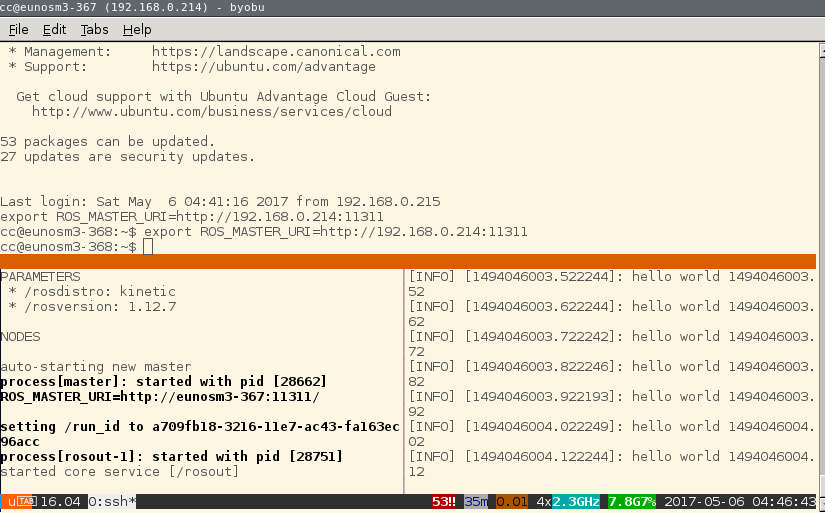
\includegraphics[width=0.75\textwidth]{images/byobu.png}}
\caption{The Multiplexed Talk-Listen Terminal}
\label{fig:byobu}
\end{figure*}

\subsection{Deployment Performance}
In general, completing the deployment process took around 500 seconds, or eight minutes and 20 seconds.  Much of that time, around five minutes, consisted of installing ROS on the cluster nodes.  Since Ansible completes each individual step of a playbook on each cluster node simultaneously, users should be able to provision a 5-, 10- or 100-node cluster as quickly as the three-node cluster used in this project, barring network communication bottlenecks, etc. 

The total amount of time needed increased when using a higher-spec Chameleon Cloud flavor, as shown in the nearby table.  However, the first portion of the process, handled by the \textit{begin} script consistently takes about 130 seconds, irrespective of the node's vCPU/RAM/HD combination.  

Furthermore, deployment failures seem to occur about 50\% of the time, independent of the CC flavor chosen.  Anecdotally, then, vCPU/RAM/HD combinations do not seem to be the first suspect to investigate with respect to failed deployments.

% \begin{table} [htbp]
%   \begin{threeparttable}
%   \centering
%   \caption{Virtual Swarm Deployment Times}
%     \begin{tabular}{ccccc}
%       \multicolumn{5}{c}{\bf Time Needed to Deploy (mean; seconds)}\\ \hline Flavor & Part 1 & Part 2 & Total & Notes\\ \hline m1.medium & 129 & 358 & 487 & 2/6 attempts succeeded \\ m1.large & 134 & 401 & 534 & 3/6 attempts succeeded \\ m1.xlarge & --- & --- & --- & no successes\\ \hline
%     \end{tabular}
%     \begin{tablenotes}
%       \small
%       \item Part 1: Consists of \textit{begin} shell script \newline  Part 2: Consists of \textit{beginAgain} shell script, which includes the Ansible playbook and installation of ROS 
%     \end{tablenotes}
%   \end{threeparttable}
% \end{table}


\subsection{Deployment Obstacles}
\paragraph{Intra-Node Communication}
In order to maintain security and enable intra-cluster communication, two of the three computer nodes must have their public ip addresses removed, i.e., disassociated, using Chameleon's browser-based graphical user interface (GUI), Horizon.  Then, and only then, the ports can be opened by applying the \textit{ros} security group to the two nodes in question (the private nodes).  Since the third node, the main node, still has a public-facing ip address, the other two nodes can be accessed via an ssh connection (\textit{ssh'ing}) to the main node and then ssh'ing to one of the private nodes.

\paragraph{Deployment Problems}
Even if a script or a user completes each step correctly to set up a controllable virtual swarm on remotely-located resources, problems still occur that cause deployment failures.  Usually, the issues can be resolved with manual intervention, so the deployment can be completed.  

\subparagraph{Adding the ROS Repository Key}
The deployment often went awry during the Ansible script step that retrieves the repository key for the ROS repo.  When the key retrieval would fail, the ROS software installation would also fail.  Obviously, if the main node lacks ROS, the simulation will not launch either.  As a workaround, the script adds the repository to each machine with the \textit{deb [trusted=yes] ...} syntax.  Using this method obviates the need for the repo key.  Although it works, applying it to repos in general creates unnecessary securirty risks.  Therefore, the workaround should be used sparingly.  

\subparagraph{Starting the Robot Simulation}
Errors while starting the simulation occurred much more frequently during the development process than the key repo problem.  In fact, approximately 50\% of tested deployments failed, almost always at the final step when launching the simulation.  

ROS prints error messages in red to the console, so they stand out.  The most common error: {\color{red} \lstinline[style=BashInputStyle]![gazebo_gui-3] process has died! }.  Sometimes, an almost identical error occurs, {\color{red} \lstinline[style=BashInputStyle]![gazebo-2] process has died! }, while other times the launch program cannot find parts of the robot model.  The latter error consists of one or both of the following: {\color{red} \lstinline[style=BashInputStyle]!Error [parser.cc:581]! }{\lstinline[style=BashInputStyle]!Unable to find uri[model://ground_plane! } and / or {\color{red} \lstinline[style=BashInputStyle]!Error [parser.cc:581]! }{\lstinline[style=BashInputStyle]!Unable to find uri[model://sun! }.  Unlike the previously-described error, this one requires manual intervention.  The user needs to enter the following commands at the terminal prompt: 

\begin{enumerate}
\setlength\itemsep{-6pt}
\item {\lstinline[style=BashInputStyle]!> killall roscore! }
\item {\lstinline[style=BashInputStyle]!> killall rosmaster! }
\item {\lstinline[style=BashInputStyle]!> killall gzclient! } 
\item {\lstinline[style=BashInputStyle]!> killall gzserver! }
\item {\lstinline[style=BashInputStyle]!> source ~/.bashrc! } 
\item {\lstinline[style=BashInputStyle]!> ./beginAgain! }
\end{enumerate}

Somewhat maddeningly, this process often needs to be completed twice before the simulation will start successfully.  If the simulation still will not start, refer to the instructions in the \textit{Initializing the Swarm Maually} section.

\subsection{Initializing the Swarm Manually}

\TODO{starting ROS and Gazebo to create the virtual environment; testing swarm interconnectivity; designating master node, etc.}

If needed the user can manually start the simulation with the commands listed below.  You will need three terminals for the three commands, so ssh into the main node three times from three separate consoles or use \textit{byobu} to split the terminal into three panes.  The command

 {\lstinline[style=BashInputStyle]!> roslaunch mybot_gazebo mybot_world.launch! } 

\parindent0pt starts the simulation.  Entering 

{\lstinline[style=BashInputStyle]!rostopic pub /robot1/cmd_vel geometry_msgs/Twist '{linear: { !} {\lstinline[style=BashInputStyle]!x: 0.2, y: 0.0, z: 0.0}, angular: {x: 0.0, y: 0.0, z: 0.1}}'! }

\parindent0pt in a free terminal will command the first robot to begin turning in a circle.  Likewise, 

{\lstinline[style=BashInputStyle]!rostopic pub /robot1/cmd_vel geometry_msgs/Twist '{linear: { !} {\lstinline[style=BashInputStyle]!x: 0.2, y: 0.0, z: 0.0}, angular: {x: 0.0, y: 0.0, z: 0.1}}'! }

moves the second robot. Alternatively, one can delete the cluster and run the deployment script again.


\section{VR Swarm Project Conclusions}

\section{VR Swarm Project Conclusions}
Automating the deployment of a virtual robot swarm on a cluster of remotely accessed computers should allow roboticists to more easily explore the benefits of collecting data from multiple sources at the same time over a give geogrpahy and timeframe.  The virtual swarm presented in this paper provides framework for obtaining those benefits. It also highlights the challenges presented with an automated deployment, including a) network communication issues like obtaining the ROS repo key for each cluster node; b) compute resource security concerns since ROS nodes bind to any available port; c) the exacting nature of the interplay between the host OS, ROS and Gazebo as shown by the high number of deployment failures despite seemingly-duplicate processes and resources.  The process developed for this project could perhaps benefit from the use of different tools and would undoubtedly benefit from a much-deeper understanding of how ROS functions.

The logical next step in the automation development process would seem to be projecting a differential drive robot started on one of the secondary nodes into the world created by ROS on the main node.  The literature the technical feasibility of the task, although the implementation may prove more difficult than expected.

\section{Supplemental Material}

% Bibliography

\bibliography{references}
 
\section*{Author Biographies}
\begingroup
\setlength\intextsep{0pt}
\begin{minipage}[t][3.2cm][t]{1.0\columnwidth} % Adjust height [3.2cm] as required for separation of bio photos.
  \noindent
  {\bfseries Matthew Lawson} received his BSBA, Finance in 1999 from
  the University of Tennessee, Knoxville. His research interests include
  data analysis, visualization and behavioral finance.
\end{minipage}
\endgroup

\appendix
\begin{description}

\item The authors would like to thank Mark McCombe for his timely and useful contribution of code snippets  to the project.  We greatly appreciate his time-saving additions to the cause.

\end{description}

\end{document}
